\documentclass[a4paper,11pt]{report}
\usepackage[T1]{fontenc}
\usepackage[utf8]{inputenc}
\usepackage[polish]{babel}
\usepackage{lmodern}
\usepackage{graphicx}

\title{Roznice w czasie realizacji algorytmu wypelniania stosu oraz listy w zaleznosci od implementacji}
\author{Arkadiusz Cyktor 200367}

\begin{document}
\maketitle

\begin{figure}
  1. Ponizszy wykres przedstawia zaleznosc czasu potrzebnego na wykonanie algorytmu od ilosci danych, dla stosu zaimplementowanego przy uzyciu tablicy. W tym przypradku tablica zwiekszana jest o jedno pole, za kazdym razem gdy dodawana jest nowa zmienna. Na wykresie widac, ze zlozonosc obliczeniowa tego algorytmu rosnie wykladniczo.
  
    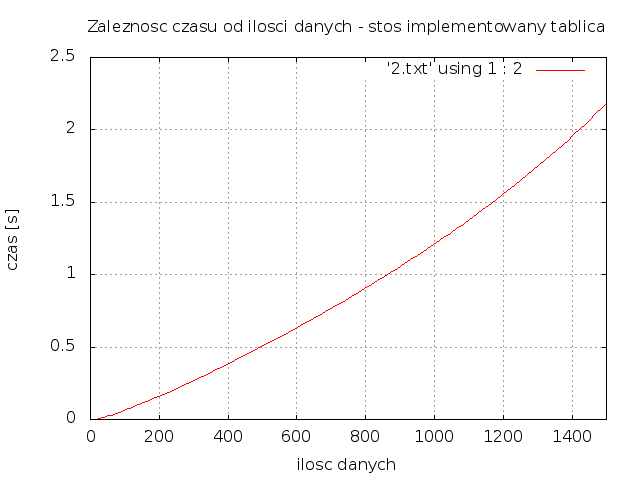
\includegraphics[scale=0.5]{./stos_tablica_o2.png}
\end{figure}

\begin{figure}
  2. Ponizszy wykres przedstawia te sama zaleznosc dla tej samej implementacji stosu, jednak tym razem rozmiar tablicy zostaje zwiekszony dwukrotnie w momencie osiagniecia przez nia zapelnienia. Z wykresu mozna wywnioskowac, ze zlozonosc obliczeniowa takiego algorytmu rowniez zwieksza sie wykladniczo.
    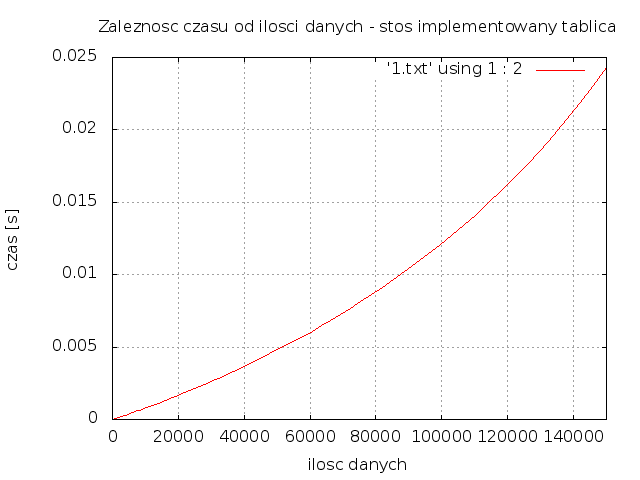
\includegraphics[scale=0.5]{./stos_tablica_o1.png}
\end{figure}

\begin{figure}
  3. Ponizszy wykres przedstawia zaleznosc czasu potrzebnego na wykonanie algorytmu od ilosci danych, dla stosu zaimplementowanego przy uzyciu listy. Ponownie widzimy, ze zlozonosc obliczeniowa rosnie wykladniczo.
    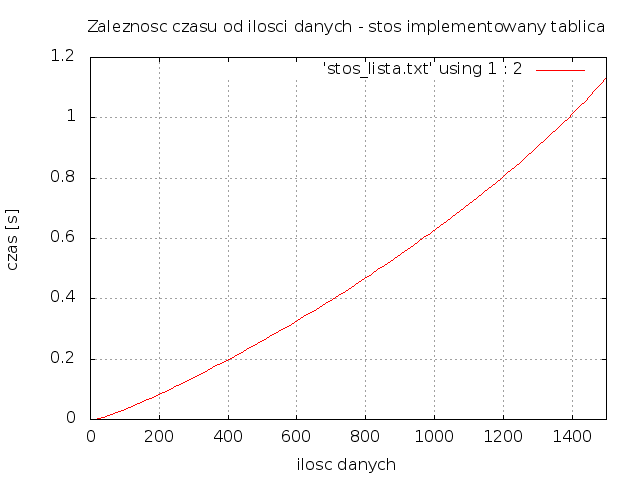
\includegraphics[scale=0.5]{./s_stos_lista.png}
\end{figure}

\begin{figure}
  4. Ponizszy wykres przedstawia zaleznosc czasu potrzebnego na wykonanie algorytmu od ilosci danych, dla kolejki zaimplementowanej przy uzyciu tablicy. Zlozonosc rosnie wykladniczo.
    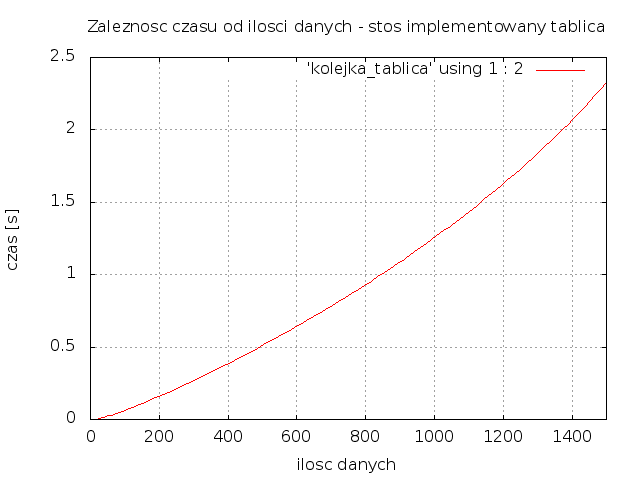
\includegraphics[scale=0.5]{./s_kolejka_tablica.png}
\end{figure}

\begin{figure}
  5. Ponizszy wykres przedstawia zaleznosc czasu potrzebnego na wykonanie algorytmu od ilosci danych, dla kolejki zaimplementowanej przy uzyciu listy. Zlozonosc rosnie wykladniczo.
    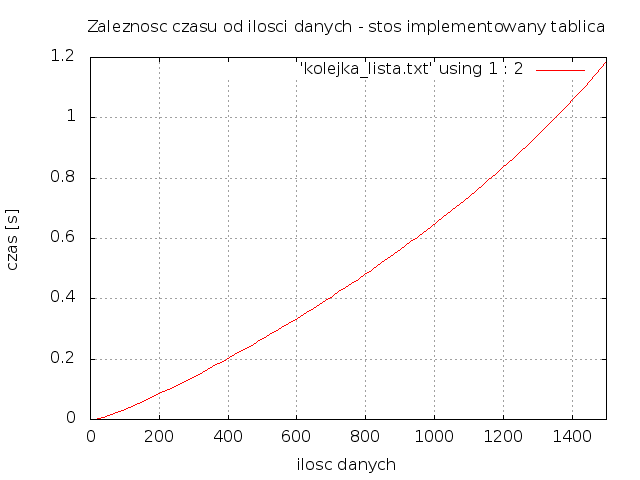
\includegraphics[scale=0.5]{./s_kolejka_lista.png}
\end{figure}

\begin{figure}
    Wnioski:
\end{figure}

\begin{figure}
    - Porownanie dwoch pierwszych wykresow pokazuje, ze dwukrotne zwiekszanie tablicy jest lepszym rozwiazaniem, przy pracy na duzej ilosc danych, niz rozszerzanie jej o pojedyncze pola. Mimo, ze zlozonosc obu rozwiazan rozne wykladniczo, to jednak przyrost ten jest znacznie mniejszy w przypadku drugiej metody, wymaga jednak ona znacznie wiecej pamieci.
\end{figure}

\begin{figure}
    - Mozemy zauwazyc, ze implementacja stosu przy pomocy listy osiaga lepsze wyniki do tych, ktore uzyskalismy podczas testowania implementacji tablicowej z powiekszaniem o jeden, pomimo faktu, ze lista rowniez jest powiekszana o jeden element w danej chwili, jesli zachodzi taka koniecznosc.
\end{figure}

\begin{figure}
    - Implementacja kolejki przy pomocy tablicy wydaje sie byc najmniej wydajna ze wszystkich testowanych.
\end{figure}

\begin{figure}
    - Podsumowujac: lista wydaje sie byc wydajniejsza obliczeniowo niz stosowana w tym samym celu tablica.
\end{figure}

\end{document}
